\section{Neomezené operátory}
V úvodní kapitole jsme ukázali charakterizaci spojitých lineárních operátorů na Banachových prostorech: pro~$\map T:~X~\to~Y$ lineární platí \begin{align*}
    \map T \text{ je omezený} \;\Leftrightarrow\; \norm{\map T} < +\infty \;\Leftrightarrow\; \map T \text{ je spojitý} \:.
\end{align*}
V této kapitole představíme některé vlastnosti \uu{lineárních}, ale \uu{neomezených a tedy nespojitých} operátorů.
Budeme pracovat pouze na Hilbertových prostorech, kde máme k dispozici vlastnosti skalárního součinu. Ukazuje se, že jsou zde problémy se samotným definičním oborem příslušného samoadjungovaného operátoru, a dokonce i samotného operátoru $\map L$.

\begin{remark}
Místo $\map L'$ jako označení adjungovaného operátoru zde budeme používat značení $\map L^*$, abychom adjungovanost odlišili od značení derivací na prostorech funkcí.
\end{remark}


\subsection{Symetrie a samoadjungovanost}
\begin{definition}[Adjungovaný operátor]
Nechť $H$ je Hilbertův prostor, $\domain(\map L) \subset H$ je lineární podprostor a $\map L : H \to H$ je lineární operátor.
\begin{enumerate}
    \item $\domain(\map L^*) \coloneqq\{y\in\ H;\;\exists!h^*\in H,\;\innerprod{\map Lx}{y}=\innerprod{x}{h^*}\;\forall x\in\domain(\map T)\}$
    \item Je-li $\domain(\map L^*)$ neprázdná množina, definujeme adjungovaný operátor $\map L^* : \domain(\map L^*) \to H$ předpisem \begin{align*}
        \map L^* y = h^* \:.
    \end{align*}
\end{enumerate}
\end{definition}

\begin{remark}
Je-li $\domain(\map L^*) \neq \emptyset$, pak z definice ihned dostáváme \begin{align*}
    (\map L x,y)_H =(x, \map L^* y)_H \quad \text{pro všechna } x \in \domain(\map L), y \in \domain(\map L*) \:.
\end{align*}
Zatímco pro omezené (spojité) operátory je předchozí rovnost důsledkem Rieszovy-Fréchetovy věty (Věta \ref{4.Riesz-Frechet}), pro neomezené operátory je třeba tuto rovnost postulovat.
\end{remark}

Přirozeně zavádíme i pojem samoadjungovaného operátoru.

\begin{definition}[Samoadjungovaný operátor]
Operátor $\map L : \domain(\map L^*) \to H$ nazveme samoadjungovaný, jestliže \begin{enumerate}
    \item $\exists\domain(\map L^*)\neq\emptyset,\;\domain(\map L^*) = \domain(\map L)$,
    \item $\map L^* = \map L$ na $\domain(\map L^*)$.
\end{enumerate}
\end{definition}
\begin{remark}
Rovnost definičních oborů je zde velmi důležitá. Později uvidíme, že pro $\domain(\map L) \neq \domain(\map L^*)$ a $\map L = \map L^*$ na $\domain(\map L) \cap \domain(\map L^*)$ dostaneme jiné spektrální vlastnosti.
\end{remark}

Přímo z definice plyne následující lemma.
\begin{lemma}
$\domain(\map L^*)\neq\emptyset\;\Rightarrow\; \map T^*$ je lineární.
\end{lemma}


\Cviceni{Kdy je $\domain(\map T^*)\neq\emptyset$?} %TODO tohle nemá být cvičení (https://www2.karlin.mff.cuni.cz/~rokyta/vyuka/1920/ls/zoom-nmaf006/c.6_2020-04-28/worksheet.pdf str. 3)

\begin{theorem}[O existenci adjungovaného operátoru]
$\map L$ je lineární operátor s definičním oborem $\domain(\map L)$. Pak $$\domain(\map L^*)\neq\emptyset \;\Leftrightarrow\;\overline{ \domain(\map L) }= H \;.$$
\end{theorem}
\begin{proof}
Lze najít ve skriptech \textsc{Lukeš}, 11.6.
\end{proof}
\Poznamka{Nejjednodušší realizace $\overline{\domain(\map L)}=H$ se zdá být přímo $\domain(\map L)=H$. K vysvětlení toho, proč tato situace nastat nemůže se dostaneme později.}


\begin{definition}[Symetrický operátor]
$\map L : \domain(\map L) \to H$ je lineární operátor, $\overline{\domain(\map L)} = H $. Řekneme, že $\map L$ je symetrický, pokud \begin{align*}
    \innerprod{\map L x}{y}_H = \innerprod{x}{\map L y}_H \quad \forall x,y \in \domain(\map L) \:.
\end{align*}
\end{definition}
Což pro neomezené operátory není totéž, co samoadjungovanost.\footnote{
Terminologie používaná v literatuře se různí. Někteří autoři používají termínů \uv{hermitovský} vs. \uv{samoadjungovaný} (např. Lukeš, Formánek) a \uv{hermitovský} vs. samoadjungovaný (např. Černý+Pokorný, Čihák). Mnoho autorů mezi pojmy dokonce nerozlišuje, většinou z~důvodu práce na dostatečně hezkých (třeba omezených, lineárních) prostorech.}
\begin{lemma}
    \begin{equation*}
    \begin{split}
        \map L \text{ je symetrický }\Leftrightarrow\left \{
    \begin{array}{ll}
        &\domain(\map L) \subseteq \domain(\map T^*)\\
        &\map T=\map T^* \text{ na }\domain(\map T)
    \end{array}
        \right.
    \end{split}
\end{equation*}
\end{lemma}
Z toho plyne implikace \uu{$\map L$ je samoadjungovaný $\Rightarrow$ $\map L$ je symetrický}. Speciálně pak \uu{$\map L$ není symetrický $\Rightarrow$}\\ \uu{$\map L$ není samoadjungovaný}. Ta se často v praxi využívá k důkazu, že $\map L$ není samoadjungovaný, aniž je třeba hledat $\domain(\map L^*)$.

\begin{theorem}[O omezenosti symetrického operátoru na celém prostoru]
    \begin{equation*}
    \begin{split}
        \left.
    \begin{array}{ll}
        &\domain(\map L)=H\\
        &\map L \text{ je lineární a symetrický}
    \end{array}
        \right \} \Rightarrow \map T \text{ je omezený}
    \end{split}
\end{equation*}
\end{theorem}
\begin{proof}
Lze nalézt opět ve skriptech \textsc{Lukeš}, 11.10.
\end{proof}

Odtud plyne 
 \begin{equation*}
    \begin{split}
        \left.
    \begin{array}{ll}
        &\domain(\map L)=H\\
        &\map L \text{ je lineární a samoadjungovaný}
    \end{array}
        \right \} \Rightarrow \map T \text{ je omezený},
    \end{split}
\end{equation*}
tedy neomezený, samoadjungovaný operátor má $\domain(\map L)\neq H$.

Jediná možná situace pro samoadjungované neomezené operátory na $H$, je
\begin{align*}
    &\domain(\map L)\neq H,\; \overline{\domain(\map L)}=H\\
    &\domain(\map L) \text{ je lin. podprostor}.
\end{align*}
O takovém operátoru $\map T$ se říká, že je \emph{hustě definován} na H.

\Priklad{(Operátor derivování)
$H = L^2 \left( (0,1) \right),\; \domain(\map L) = \mathcal{C}^1 \left( [0,1] \right)$. Na tomto prostoru definujme $\map L f = f'$.

Víme, že $\mathcal{C}^1 \left( [0,1] \right)=L^2((0,1))$. Operátor je zřejmě lineární a neomezený.

Zkoumejme symetrii jako nutnou podmínku samoadjungovanosti. Zřejmě je \begin{align*}
    \innerprod{\map L f}{g}_{L^2} =\innerprod{f'}{g}_{L^2} = \int_0^1 f'(x) \conj{g}(x) \d x \:, \qquad \innerprod{f}{\map L g}_{L^2} = \int_0^1 f(x) \conj{g}'(x) \d x \:.
\end{align*}
Aplikujeme-li metodu per-partes, dostaneme \begin{align*}
    \int_0^1 f'(x) \conj{g(x)} \d x = \left[ f(x) \conj{g(x)} \right]_0^1 - \int_0^1 f(x) \conj{g'(x)} \d x \:.
\end{align*}
Ani v případě, že se pomocí vhodných okrajových podmínek zbavíme krajních členů, nemůže být operátor derivace $\map L$ nikdy symetrický, tedy ani samoadjungovaný, kvůli změně znaménka před integrálem.

Určíme nyní $\domain(\map L^*)$ vyšetřením množiny
\vspace*{-1cm}
\begin{align*}
\big \lbrace g \in C^1 \left( [0,1 ]\right) : \exists !h^* \in L^2\left(
(0,1)\right) \text{ tak, že }
\overbrace{\innerprod{\map L f}{g}_{L^2}=\innerprod{f}{h^*}_{L^2}}%
^{[f\conj{g}]_0^1-\int\limits_0^1f\conj{g'}=\int\limits_0^1f\conj{h^*}\quad
(\star)} \;\forall f \in C^1 \left( [0,1 ]\right)  \big \rbrace \:,
\end{align*}

přičemž platnost rozpisu dle Per-Partes vyžadujeme pro $\forall f\in\mathcal{C}^1([0,1])$.

Volbou speciálních funkcí $f$ zjistíme nutné podmínky.
\begin{itemize}
    \item[1.] Zvolíme funkci $f$ jako na obrázku:

            {\hfill 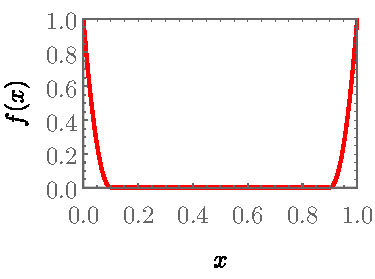
\includegraphics{img/operator_derivovani_1.pdf} \hfill}

        Při dosazení těchto $f_\epsilon$ do $(\star)$ a provedením limity $\epsilon\rightarrow0^+$ dostaneme $[f \conj{g}]_0^1=0$.
    \item[2.] Volbou $f_\delta$, definovaného obrázkem jako
    \item[3.] Zvolíme funkci dle jednoho z obrázků

            {\centering 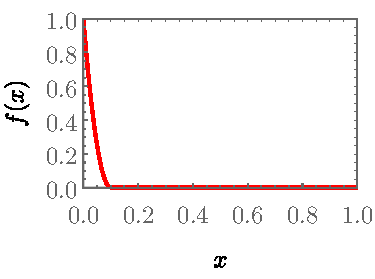
\includegraphics{img/operator_derivovani_2.pdf} \quad 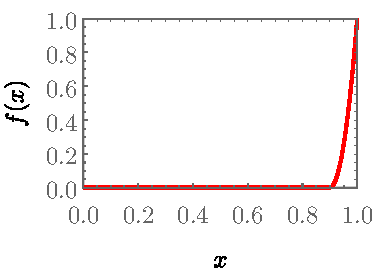
\includegraphics{img/operator_derivovani_3.pdf}}

        dostaneme podmínku $g(0)=g(1)=0$. To je první zpřesnění, ze kterého plyne $$\domain(\map L^*)\subseteq\{g\in\mathcal{C}^1([0,1]),\;g(0)=g(1)=0\}$$
\end{itemize}
}

\newpage

\lboxed{%
\phantom{\fbox{\textbf{Příklad}}} \;
\parbox[t]{\textwidth - 7em}{%
\begin{itemize}
    \item[4.] $(\star)$ se tedy redukuje na
        \begin{align*}
            -\int\limits_0^1f\conj{g'} &=\int\limits_0^1f\conj{h^*}\\
            \int\limits_0^1f(\conj(g'+h^*) &=0\;\;\forall f\in\mathcal{C}^1([0,1]).
        \end{align*}
        Odtud (z du Bois-Reymondova lemmatu) plyne $h^*$ je s.v. rovno spojité funkci $-g'$. Lze ho tedy považovat za spojité.
\end{itemize}

Nalezli jsme $h^*$, tedy není třeba dále modifikovat $\domain(\map L^*)$. Máme
\begin{align*}
   \domain(\map L^*) &= \{ g\in\mathcal{C}^1([0,1]),\;g(0)=g(1)=0\}\\
   \map L^*g&=-g^*
\end{align*}
Evidentně $\map L\neq \map L^*$, navíc i $\domain(\map L^*)\subsetneqq \domain(\map L)$.

\begin{align*}
     -\int_0^1 f \conj{g'} \d x = \int_0^1 f \conj{h^*} \d x
\end{align*}
Po převedení obou integrálů na pravou stranu a s použítím Du-Bois-Reymondova lemmatu dostáváme požadavek
\begin{align*}
     h^* = -g' \quad \text{skoro všude} \:.
\end{align*}
(Protože hledáme řešení na třídě $C^1$ a tam patří funkce $g$, uvažujme pouze
$h^* \in L^2\left( (0,1)\right) \cap C^1 \left(  [0,1] \right)$.)

Celkově jsme dostali
\begin{align*}
\domain(\map L^*) = \left \lbrace g \in C^1 \left( (0,1)\right) \cap C^1 \left(  [0,1] \right) :  g(0)=g(1)=0 \text{ a zároveň } \map T^* g=-g^* \right \rbrace \:.
\end{align*}

Povšimněme si, že $\map L \neq \map L^* $ a navíc $\domain(\map L^*)
\subset \domain(\map L)$, ale $\domain(\map L^*) \subset
\domain(\map L)$.
}}




\Priklad{ (Modifikovaný operátor derivování)
Pro samoadjungovanost operátoru derivace je třeba modifikovat jak $\map L$ (aby vyšlo $\map L^*=\map L$), tak $\domain(L)$ (aby byl $\domain(L^*)=\domain(\map L)$).
Myšlenka pro modifikaci vychází z~pozorování
$$\map Lf=f' \;\Rightarrow\;\map L^*f=-f',$$
přičemž přebývající znaménko je třeba \uv{rozpůlit mezi $\map L$ a $\map L^*$}. Definujme tedy
\begin{align*}
    \map L f \coloneqq i f' \quad \text{ na } L^2 \left( (0,1) \right).
\end{align*}
Jelikož nutnou podmínkou pro samoadjungovanost je symetrie, bude pro symetrii potřeba mít v~$\domain(\map L)$ správně podchyceny okrajové podmínky. Uvažujme tři možnosti
\begin{enumerate}
    \item $\domain(\map L_1) = L^2 \left( (0,1) \right) \cap  C^1 \left( [0,1] \right)$,
    \item $\domain(\map L_2) = L^2 \left( (0,1) \right) \cap  C^1 \left( [0,1] \right) \cap \{ f(x): f(0)=f(1)\}$,
    \item $\domain(\map L_3) = L^2 \left( (0,1) \right) \cap  C^1 \left( [0,1] \right) \cap \{ f(x): f(0)=f(1)=0\}$
\end{enumerate}
a tři restrikce \begin{align*}
    \map L_1 = \map L\rvert_{\domain(\map L_1)} \:, \qquad \map L_2 = \map L\rvert_{\domain(\map L_2)} \:, \qquad \map L_3 = \map L\rvert_{\domain(\map L_3)} \:.
\end{align*}
Symetrie pak plyne z:
$$\innerprod{\map Lf}{g}=\int\limits_0^1if'\conj{g}=\underbrace{[if\conj{g}]_0^1}_{(\star)}-i\int\limits_0^1f\conj{g}' = \underbrace{[if\conj{g}]_0^1}_{(\star)}+\int\limits_0^1f\conj{ig'}$$
$$
(\star)  \begin{cases}
= 0\;\; \text{pro } f,g\in \domain(L_2) \text{, nebo } f,g\in \domain(L_3)\\
\neq0 \;\; \text{pro }f,g\in \domain(L_1),
\end{cases}
$$
z čehož plyne, že symetrické jsou pouze $\map L_2, \map L_3$ a $\map L_1$ symetrický není. Jako cvičení si zkuste ukázat
\begin{itemize}
    \item $\domain(\map L_1^*)=\domain(\map L_3)\subsetneqq\domain(\map L_1)$ (další potvrzení toho, že $\map L_1$ ení symetrický)
    \item $\domain(\map L_2^*)=\domain(\map L_2)$ (tj. může být samaoadjungovaný)
    \item $\domain(\map L_3^*)=\domain(\map L_1)\subseteq \domain(\map L_3)$ (tj. potvrzení symetrie, ale zároveň důkaz, že $\map L_3$ \emph{není} samoadjungovaný.)
\end{itemize}
Jediný kandidát na samoadjungovanost je $\map L_2$, který je symetrický a splňuje $\domain(\map L_2^*)=\domain(\map L_2)$. Zbývá ověřit, že $\map L=\map L^*$ na tomto definičním oboru. To plyne podobně jako v předchozím příkladu. Ze symetrie máme
$$\innerprod{\map Lf}{g} = \overset{\text{na} \domain(\map L_2^*)}{\innerprod{f}{\map Lg}\quad=\quad\innerprod{f}{h^*}}\quad\forall f\in\mathcal{C}^1([0,1])\quad \text{atd.}$$

\uu{Závěr:} $\map L_1$ není symetrický (ani samoadjungovaný), $\map L_3$ je symetrický (ale není samoadjungovaný) a~$\map L_2$ je samoadjungovaný. Vidíme, že i v případě $\domain(\map L)$ se okrajové podmínky \uv{rozdělily} mezi $\domain(\map L_2)$ a $\domain(T_2^*)$.
}


\begin{remark}
Připomeňme kvantověmechanický operátor hybnosti \begin{align*}
    \hat p = -i \hbar \dd{}{x} \quad \text{definovaný na } L^2(\R) \cap C^1(\R) \:.
\end{align*}
Modifikací předchozího příkladu snadno zjistíme, že operátor definovaný na takové množině je symetrický, ale není obecně samoadjungovaný. Je si třeba uvědomit, z jakého prostoru bereme vlastní vektory. Pokud bychom se snažili nalézt řešení rovnice \begin{align*}
    -i \hbar \dd{\psi}{x} = k \psi(x) \:,
\end{align*}
zjistili bychom, že vlastní funkce \begin{align*}
    \psi(x, k) = C e^{\frac{ik}{\hbar} x}
\end{align*}
nepatří do $L^2(\R)$. Z hlediska spektrální analýzy tedy nemá operátor hybnosti žádné vlastní vektory.
\end{remark}



\subsection{Spektrum neomezených operátorů}

V případě omezených operátorů hrály zásadní roli pro charakter spektra následující třídy operátorů: \begin{itemize}
    \item Samoadjungované operátory: jsou zavedeny i pro neomezené operátory, avšak komplikovanějším způsobem.
    \item Kompaktní operátory: jsou podmnožinou omezených operátorů. Jejich roli v množině neomezených operátorů částečně převezme třída uzavřených operátorů.
\end{itemize}

\begin{definition}[Uzavřený operátor]
$\map L : \domain(\map L) \to H$ je lineární operátor hustě definovaný na $H$.  Řekneme, že $\map L$ je uzavřený, pokud pro $x_n\in\domain(\map L)$:
 \begin{equation*}
    \begin{split}
        \left.
    \begin{array}{ll}
        x_n&\rightarrow x\in H\\
        \map Lx_n&\rightarrow g \in H
    \end{array}
        \right \} \Rightarrow x\in \domain(\map L),\; \map Lx=g,
    \end{split}
\end{equation*}
\end{definition}
nebo-li $\map L$ má \emph{uzavřený graf}: $[x_n,\map Lx_n]\rightarrow [x,g]\;\Rightarrow g=\map L x$ a $[x,\map Lx]\in \text{ graf}$. Slovně lze tuto vlastnost definovat tak, že \uv{konverguje-li posloupnost vzorů a současně i posloupnost obrazů, pak musí limita obrazu být zobrazenou limitou vzoru.}

Dále jsme u omezených operátorů studovali, zda jsou prosté a na. Tato otázka má smysl i u neomezených operátorů. Konečně jsme takové studovali spojitost inverzních operátorů. Touto otázkou se, celkem překvapivě, má smysl zabývat i v této kapitole. \uu{Zjistili jsme tedy, že nespojité lineární operátory v nekonečné dimenzi mohou být} \uu{uzavřené, ač jsou nespojité a mohou mít spojitou inverzi}.

\begin{theorem}[O spektrálních vlastnostech neomezených operátorů]
$\map L : \domain(\map L) \to H$ je lineární operátor hustě definovaný na $H$. Pak 
\begin{enumerate}
    \item $\overline{\mathcal{R}(\map L)} = H\;\Rightarrow\; \map L$ prostý a na $\mathcal{R} (\map L)$.
    \item $\mathcal{R}(\map L) = H\;\Rightarrow\; \map L$ je prostý, na H, samoadjungovaný a $\map L^{-1}$ je spojitý.
    \item $\map L^{-1}$ je spojitý $\Leftrightarrow\;\map L$ je prostý, na $H$ a uzavřený.
\end{enumerate} 
\end{theorem}
\begin{proof}
Viz např.  \textsc{Rudin}: Functional analysis, 13.11 a dál.
\end{proof}

\begin{definition}[Resolventa, spektrum operátoru] \qquad
\begin{itemize}
    \item Resolventa $L\equiv \Res(\map L) \coloneqq \{ \lambda\in \C,\;\map L_{\lambda} \text{ prostý, na }H,\;\map L_\lambda^{-1}$ spojitý\}.
    \item Spektrum $\map L\equiv \Sp(\map L) \coloneqq \C \setminus \Res\, \map L = \begin{cases}
\text{bodové spektrum (vl. č.)} \coloneqq \{\lambda\in\C,\;\map L_\lambda \text{ prostý, na } H,\; \map L_\lambda^{-1} \text{ spojitý}\}\\
\text{zbytek}
\end{cases}$
\end{itemize}
\end{definition}

\begin{remark}
Spektrum neomezeného operátoru může být jakákoli neomezená podmnožina $\C$, včetně celého $\C$.
\end{remark}

\uu{Vlastnosti spektra lineárních neomezených operátorů $\map L$ na $H$} 
\begin{enumerate}
    \item $\map L$ je uzavřený $\Rightarrow \Sp(\map L)$ je uzavřená množina v $\C$.
    \item $\map L$ uzavřený a symetrický, pak nastane právě jedna z následujících situací: \begin{enumerate}
        \item $\Sp(\map L) = \C$,
        \item $\Sp(\map L) = \{ \lambda \in \C,\; \mathrm{Im}\, \lambda \geq 0 \}$,
         \item $\Sp(\map L) = \{ \lambda \in \C,\; \mathrm{Im} \, \lambda \leq 0 \}$,
          \item $\Sp(\map L)$ je uzavřená podmnožina $\R$.
    \end{enumerate}
    Pouze v bodu d) je $\map L$ samoadjungovaný, jinak je pouze symetrický.
    \item Je-li $\map L$ symetrický a má reálná vlastní čísla (případně pokud je uzavřený a samoadjungovaný), pak jsou vlastní vektory příslušející různým vlastním číslům na sebe kolmé.
\end{enumerate}


\begin{remark}\qquad
\begin{enumerate}
    \item Druhá část předchozí věty ukazuje velkou odlišnost mezi samoadjungovaným a symetrickým operátorem. Neomezený symetrický operátor může obsahovat prvky z nebodového spektra, které nejsou reálné. U samoadjungovaného operátoru taková situace nemůže nastat.
    \item Vlastních čísel i vektorů může mít neomezený operátor obecně nespočetně mnoho. Odvětví matematiky zabývající se touto problematikou se nazývá spojitý funkcionální kalkulus, užívající obecnějšího integrálu namísto sumace při rozkladu prvků do vlastních vektorů.
    \item V teorii o neomezených operátorech nemáme apriori věty o úplnosti zadaného systému. V konkrétních případech je třeba jejich úplnost dokazovat případ od případu.
\end{enumerate}
\end{remark}











\pagebreak